\documentclass{article}
\usepackage{fullpage}
\usepackage{physics}
\usepackage{authblk}
\usepackage{indentfirst}
\usepackage{commath}
\usepackage{graphicx}
\usepackage{float}
\usepackage{subfig}
\usepackage{amsmath}
\usepackage{bm}
\usepackage[utf8]{inputenc}
\usepackage[T1]{fontenc}

\author{Hunter Belanger}

\title{L'Analyse Préliminaire sur le Delta Tracking}
\date{}

\begin{document}
	\maketitle
	
	\section{Le Système à Modeler}
	Le système qui sera analysé pendant ce travail est un réacteur plaque fini et réfléchi. Pour la simplicité, l'épaisseur du cœur était choisi d'être 40$cm$, avec un réflecteur de 30$cm$ à chaque coté, qui ensemble fait un réacteur avec une épaisseur de 100$cm$. Un diagramme du système se trouve en Figure~\ref{fig:réacteur}.
	
	\begin{figure}[H]
		\centering
		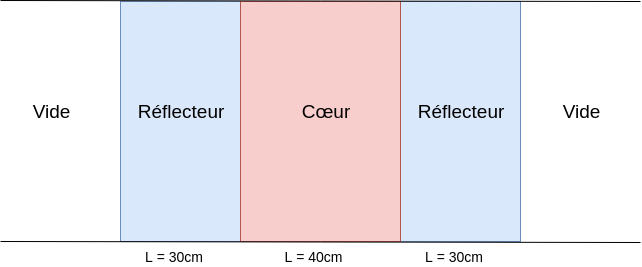
\includegraphics[scale=0.45]{reacteur.png}
		\caption{Réacteur plaque fini et réfléchi, utilisé dans tous les simulations qui se trouve dans ce travail.}
		\label{fig:réacteur}
	\end{figure}
	
	L'approximation de deux groupes est aussi utilisé. L'index 1 représente les neutrons rapides et l'index 2 représente les neutrons thermiques. Les sections efficaces pour chaque matière et chaque énergie sont présentés en Tables 1 et 2.
	
	\begin{table}[H]
		\centering
		\begin{tabular}{|c|c|c|}
			\hline
			\textbf{Sections Efficaces} & \textbf{Réflecteur} & \textbf{Cœur} \\ 
			\hline \hline
			$\Sigma_{t_1}$ & 0,295 & 0,276 \\
			$\Sigma_{t_2}$ & 2,1 & 1,063 \\
			\hline
			$\Sigma_{a_1}$ & 0,0004 & 0,012 \\
			$\Sigma_{a_2}$ & 0,02 & 0,121 \\
			\hline
			$\Sigma_{f_1}$ & 0,0 & 0,00339 \\
			$\Sigma_{f_2}$ & 0,0 & 0,074 \\
			\hline
			$\nu_1$ & 0,0 & 2,5 \\
			$\nu_2$ & 0,0 & 2,5 \\
			\hline
		\end{tabular}
		\caption{Les sections efficaces pour le réacteur (en unités de $cm^{-1}$), sauf les matrices de diffusion.}
	\end{table}
	
	\begin{table}[H]
		\centering
		\subfloat[Réflecteur]{
			\begin{tabular}{|c | c | c |}
				\hline
				 & \textbf{à 1} & \textbf{à 2} \\
				 \hline
				 \textbf{1} & 0,2456 & 0,049 \\
				 \hline
				 \textbf{2} & 0,0 & 2,08 \\
				 \hline				
			\end{tabular}
		}
		\hspace{50pt}
		\subfloat[Cœur]{
			\begin{tabular}{|c | c | c |}
				\hline
				& \textbf{à 1} & \textbf{à 2} \\
				\hline
				\textbf{1} & 0,25 & 0,014 \\
				\hline
				\textbf{2} & 0,0 & 0,942 \\
				\hline				
			\end{tabular}
		}
		\caption{Les matrices de diffusion, $\Sigma_{j\rightarrow i}$, pour le réacteur (en unités de $cm^{-1}$).}
	\end{table}
	
		\subsection{Point de Comparaison: MCNP et OpenMC}
		Deux solutions pour ce système ont été établi avec MCNP et OpenMC. Ces deux logiciel ont fourni leurs valeurs pour la criticité. MCNP a aussi calculé le flux des neutrons dans chaque groupe. Ces calculs ont été effectués avec 1000000 histoire, et 1015 générations (les premières 15 étaient ignorées).
		
		\begin{table}[H]
			\centering
			\begin{tabular}{|c|c|}
				\hline
				\textbf{Logiciel} & \bm{$k_{eff}$} \\
				\hline
				\hline
				MCNP & 1.00914 $\pm$ 0.00002 \\
				\hline
				OpenMC & 1.00915 $\pm$ 0.00002 \\
				\hline
			\end{tabular}
			\caption{Les valeurs de la criticité obtenus pour ce système.}
			\label{tab:crit}
		\end{table}
		
		La criticité de MCNP en Table~\ref{tab:crit} sera considérée le valeur principale, représentant ce que nous considérons la vrais solution.
		
		\begin{figure}[H]
			\centering
			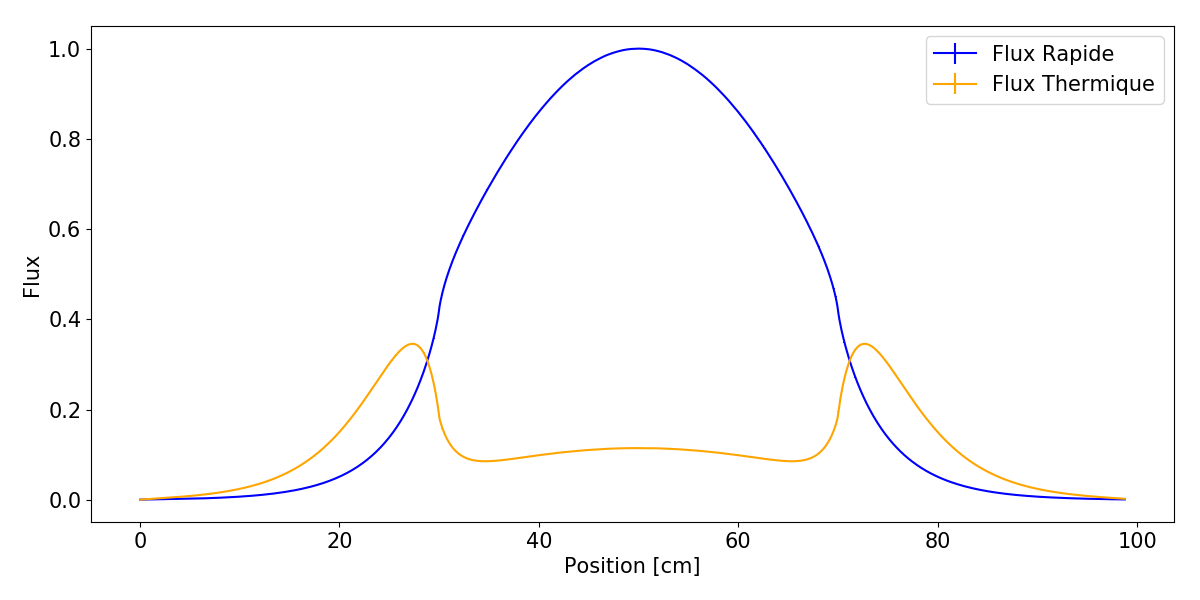
\includegraphics[scale=0.5]{mcnp_flux.png}
			\caption{text}
			\label{fig:mcnp_flux}
		\end{figure}
	
		\begin{figure}[H]
			\centering
			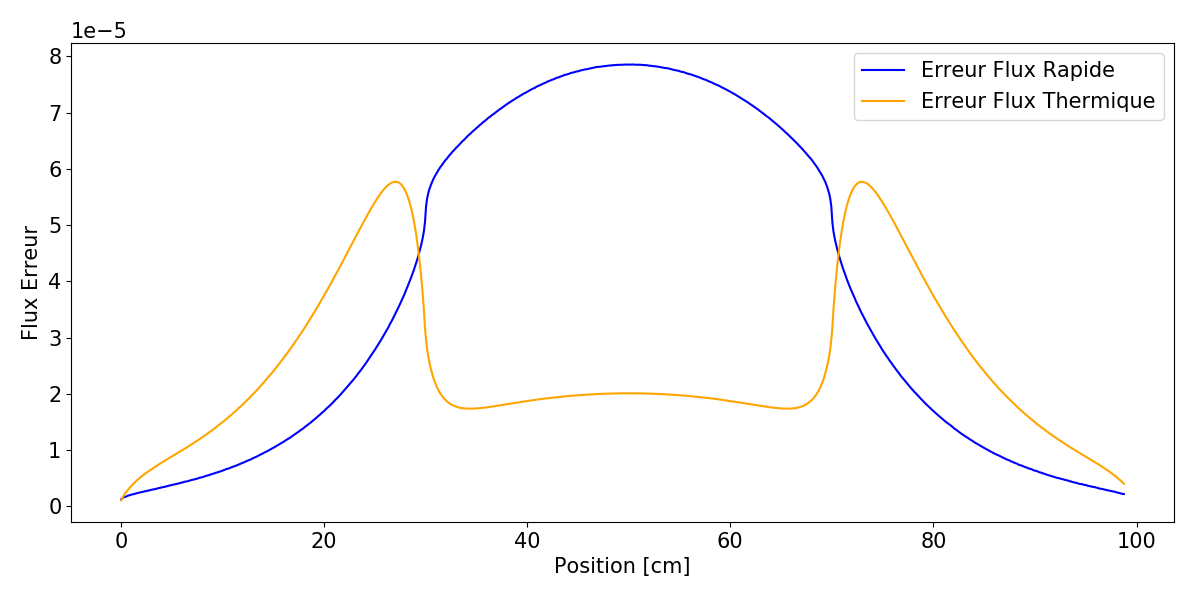
\includegraphics[scale=0.5]{mcnp_flux_erreur.png}
			\caption{text}
			\label{fig:mcnp_flux_erreur}
		\end{figure}
	
		\subsection{Méthodes des Calculs}
			Voici expliqué les moyennes utiliser pour faire tous les calculs du flux, de l'entropy, et du FOM. Les codes suivant que j'ai écrits ont utilisé les mêmes méthodes pour que la seule différence entre leurs résultats soient à cause de leur méthode de tracking (ray tracing, delta-tracking, etc.).
			\subsubsection{Flux}
			Pour calculer le flux, le réacteur a été divisé en 1000 boîte, chacune d'une épaisseur de 0,1$cm$. Chaque fois un neutron a une collision, le valeur du flux pour la boîte correspondant à la position de neutron est augmenté par la quantité
			\begin{equation*}
				F_{E,b} \quad += \quad \frac{w}{\Sigma_t(x)}
			\end{equation*}
			où $E$ est l'énergie du neutron (rapide ou thermique), $b$ est la boîte correspondant à la position de la collision ($x$), et $w$ et le poids du neutron. Il n'est pas nécessaire de normaliser par la taille de la boîte, comme chaque boîte dans ces simulations ont la même épaisseur, et nous ne considèrerons que le flux normalisé. 
			
			\subsubsection{Entropy}
			D'une façon similaire à celle du flux, pour calculer l'entropy de chaque génération, le cœur est divisé en 200 boîte d'une épaisseur de 0,2$cm$. Le nombre de neutrons dans boîte $b$ au début de la génération est $N_b$, et l'entropy pour la génération est calculé avec
			\begin{equation*}
				H = \sum_{b} N_b \log_2(N_b)
			\end{equation*}
			où je suppose qu'il n'y a aucune boîte sans neutrons. Cela est une supposition valide dans ce cas où il n'y a qu'une seule région qui produit les neutrons, et il y en a beaucoup en chaque générations.
			
			\subsubsection{Figure of Merit}
			Le Figure of Merit (FOM) est calculé avec la formule suivante:
			\begin{equation*}
				FOM = \frac{1}{T\big(\frac{\sigma}{k_{avg}}\big)^2}
			\end{equation*}
			où $T$ est le temps en seconds depuis la première génération qui n'est pas ignoré a commencée, $\sigma$ est l'incertitude de la moyenne de la criticité, $k_{avg}$.
		
	\section{La Méthode de Ray Tracing}
	
	
	
\end{document}